\chapter{Introduction}

With the emergence of new sequencing systems genomic data is being generated at an unprecedented rate.Almost two decades back \textbf{The Human Genome Project} took 13 years and over 3 billion dollars to sequence the entire human genome whereas the same information can be sequenced today in under an hour for 1000 dollars.This rapid improvement in sequencing genomic data has improved the availability of high resolution genomics data and has helped researchers in answering a wide range of biological questions.


% reference to https://www.genome.gov/human-genome-project/Completion-FAQ


An important field in biological research where genomic data is extensively used is comparative genomics.It involves comparing genomic information between different species to understand their similarity.A genome of an organism consists of its complete set of DNA in the form of a series of genes where every gene is a sequence that is responsible for one or more traits in that organism.Comparing genomic sequences between two different organisms can help researchers in understating their evolutionary relationship as similar sequences can often mean that the genes have the same function.Such similar sequences are referred to as homologous sequences and they indicate shared ancestry.As organism evolve overtime and diversify into different species they retain parts of their DNA from their common ancestor.The study of these conserved homologous regions is called \textbf{Synteny}. 

While a huge part of comparing large scale genomic sequences is purely computational and thus can be automated human judgement is still vital in syteny analysis.Visual data exploration for example can help researchers in easily identifying similarities among large scale genomes as humans are intuitively good at picking out patterns in pictures and visuals.Synteny visualization commonly involves visualizing genomes at the whole genome level or the individual chromosome level and representing similar genes either by connected links or similar colored regions.Syntenic data analysis can often be an iterative process where researchers visualize computational results multiple times under various parameters such as the size and orientation of similar genes based on a given biological hypothesis.

The choice of visual encoding in the representation of syntenic relationship is dependant on the kind of analysis that is being done by the researchers.Certain graphical representations like dot plots where every conserved gene is represented as a point on a two dimensional matrix, are useful in analyzing extremely large genomes in a single representation as shown in Figure \ref{fig:ch_1_dot_plot} while other representations like linear horizontal plots where syntenic links are represented as coloured ribbons connecting similar regions are useful in performing a more in depth analysis as the conserved regions are more visually prominent.Additionally Circos plots which use a circular ideogram layout as shown in Figure \ref{fig:ch_1_circos_plot} are also used by researchers commonly in publications as they can be aesthetically pleasing.

With such varied graphical representations, arriving at the right form of visualization can be difficult and any system that offers only a single kind of visual encoding can become limited in its usability for a wide range of biological scenarios.Apart from looking at synteny in multiple representations researchers are also often interested in  investigate specific conserved regions further and thus needing the visualization system to be adaptive based on the genomic scale of interest.Thus visualizations systems need to go beyond acting as basic chart generating systems and instead offer a rich interactive experience where researchers can explore sequences from the whole genome level all the way down to the individual gene level in multiple graphical representations.

A key part of every visualization system is the data that drives it and genomic data owing to its large volume, is being increasingly managed and distribution through several online databases like NCBI and genBank.This rapid dissemination of data across the internet has created a need for visualization systems to be easily available across the web so researchers can collaborate and share their work.


\begin{figure}
\centering
\begin{minipage}{.5\textwidth}
  \centering
  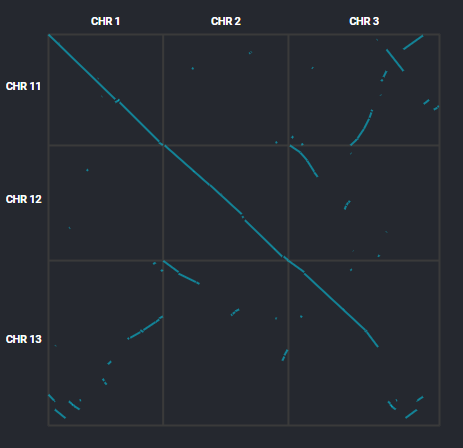
\includegraphics[width=.75\linewidth]{images/ch_1_dot_plot.PNG}
  \captionof{figure}{Dot plot}
  \label{fig:ch_1_dot_plot}
\end{minipage}%
\begin{minipage}{.5\textwidth}
  \centering
  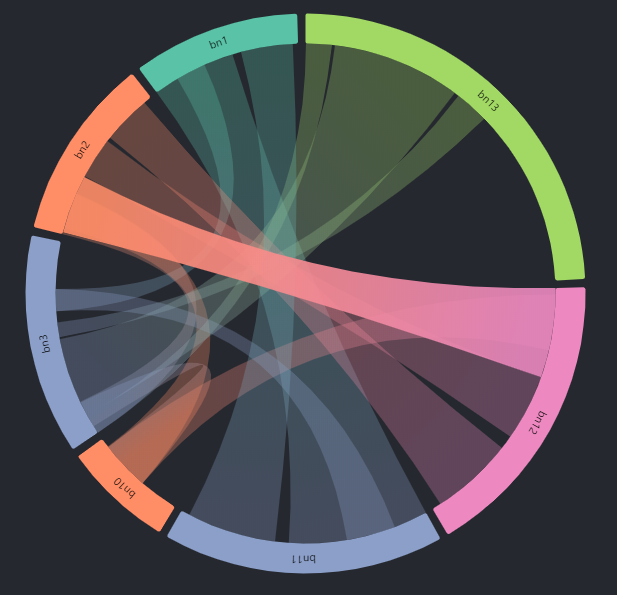
\includegraphics[width=.75\linewidth]{images/ch_1_circos_plot.PNG}
  \captionof{figure}{Circos Plot}
  \label{fig:ch_1_circos_plot}
\end{minipage}
\end{figure}


\section{Problem and Motivation}

The problem addressed in this thesis is: \textit{existing synteny tools are limited in their accessibility, offer little or no interactive experience and aren't integrated with the existing synteny detection tools to offer a seamless experience.}

Owing to the complexity involved in generating visualizations of large scale genomes, synteny visualization tools are largely command line based or stand alone programs limited to working in specific operating systems.This combined with the steep learning curve in using these systems means that a large set of these tools aren't accessible to the wider science community.Of the few online visualizations systems that exist, most act as simple chart generation systems instead of offering researchers chance to explore their datasets.This has largely pushed visualization into the report generation stage instead of the  iterative hypothesis testing phase of the research cycle.

Understanding genomic conservation is crucial for researchers as it has applications in a wide variety of scenarios such as predicting whole genome duplication events,sequencing extremely large genome sequences like wheat and classifying the proximity of different species in their evolutionary history.
While visualization systems are important as report generating tools that can create publication ready charts they need to move to earlier stages of the stages of the research cycle to accelerate the process of hypothesis testing.
Researchers should have the ability to interact with their datasets and change parameters in real time to see their results in easily understandable visual,
which in turn can let researchers explore a wide range of biological scenarios in a short span of time.
% refer vgsc

\section{Solution}

To address the lack of proper analysis tools in syteny research we developed \textbf{SynVisio} an online syteny visualization toolkit that can assist researchers in exploring genomic conservation.

\textbf{SynVisio} can directly work with results of existing syteny detecting tools like MCScanX and DAGChainer and can visualize conservation in multiple representations.It works in two modes,the basic synteny analysis mode lets users compare chromosomes in the same genome or between two genomes and the information is visualized as Horizontal linear plots,Dot plots or both.For visualizing synteny across several genomes simultaneously \textbf{SynVisio} offers a Multi-level analysis mode where synteny is visualized in stacked horizontal plots or Hive plots.\textbf{SynVisio} offers a rich interactive experience by letting users switch graphs in real time and explore data from genome level all the way down to the individual gene level.Users can do this by simply clicking on any two chromosomes when looking at a visualization in the genome level and then further step down from the individual chromosome level by clicking on a particular gene block to look at its constituent  genes and their orientation. Additionally users also have the ability to annotate their charts with additional genomic data in the form of tracks above the genomes or chromosomes which can be visualized as heat-maps,histograms or scatter-plots.

By default \textbf{SynVisio} lets users select the chromosomes that they wish to explore and then visualizes the conserved gene blocks in a dashboard that shows both the Horizontal linear plot and a Dot plot along with a filter panel where users can refine the results using a slider based on the level of similarity and the number of contiguous genes in a conserved block.
As users explore the synteny results \textbf{SynVisio} offers them the ability to records their interactions as snapshots which can be revisited or reset giving the ability to explore multiple scenarios and switch between them.The system also indexes all the conserved genes in the browser thus letting users quickly lookup genes by their gene IDs to see which conserved blocks they belong to.Finally \textbf{SynVisio} offers users the ability to download all the charts in transform and scale invariant vector graphics for research publication.

\section{Steps to the Solution} 
There were several steps involved designing a system that could let researchers explore syteny through an easily accessible web based based tool.

\section{Evaluation}

\section{Contribution}

\section{Thesis Outline}